% Copyright (c) 2020 Carl Martin Ludvig Sinander.

% This program is free software: you can redistribute it and/or modify
% it under the terms of the GNU General Public License as published by
% the Free Software Foundation, either version 3 of the License, or
% (at your option) any later version.

% This program is distributed in the hope that it will be useful,
% but WITHOUT ANY WARRANTY; without even the implied warranty of
% MERCHANTABILITY or FITNESS FOR A PARTICULAR PURPOSE. See the
% GNU General Public License for more details.

% You should have received a copy of the GNU General Public License
% along with this program. If not, see <https://www.gnu.org/licenses/>.

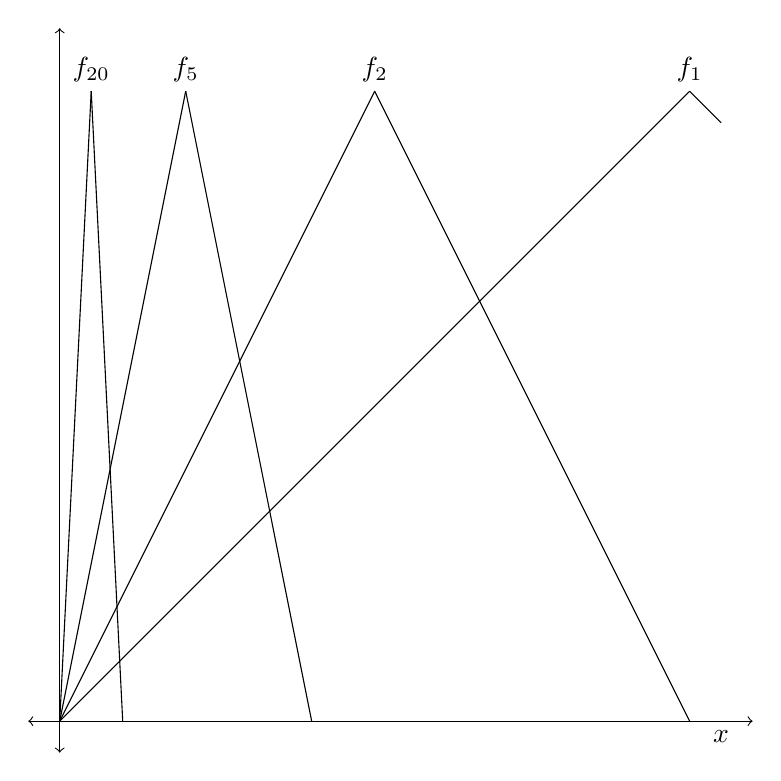
\begin{tikzpicture}[scale=8]
	
	% up
	\draw[-] (0,0) -- (1/01,1);
	\draw[-] (0,0) -- (1/02,1);
	\draw[-] (0,0) -- (1/05,1);
	\draw[-] (0,0) -- (1/20,1);

	% down
	\draw[-] (1/01,1) -- (1.05,0.95);
	\draw[-] (1/02,1) -- (2/02,0);
	\draw[-] (1/05,1) -- (2/05,0);
	\draw[-] (1/20,1) -- (2/20,0);

	% function
	\draw (1/01,1) node[anchor=south] {$f_{1}$};
	\draw (1/02,1) node[anchor=south] {$f_{2}$};
	\draw (1/05,1) node[anchor=south] {$f_{5}$};
	\draw (1/20,1) node[anchor=south] {$f_{20}$};

	% axis labels
	\draw (1.05,0) node[anchor=north] {$x$};

	% axes
	\draw[<->] (-0.05,0) -- (1.1,0);
	\draw[<->] (0,-0.05) -- (0,1.1);

\end{tikzpicture}